\documentclass[10pt,letterpaper]{article}

  %%%%%%%%%%%%%%%%%%%%%%%%%%%%%%%%%%%%%%%%%%%%%%%%%%%%%%%%%%%%%%%%%%%%%%%%%
  % \setallmargins{1in}

  \usepackage[margin=1in]{geometry}

  \usepackage{fancyhdr,lastpage}
  \pagestyle{fancy}

  \fancyhead{}
  \fancyfoot{}

  \renewcommand{\headrulewidth}{0.5pt}
  \renewcommand{\footrulewidth}{0pt}

  \rhead{Kesari}
  \lhead{NSF Proposal, Fall 2017}
  \cfoot{\thepage}
  %

  %%%%%%%%%%%%%%%%%%%%%%%%%%%%%%%%%%%%
  \newcommand{\required}[1]{\section*{\hfil #1\hfil}}
  \renewcommand{\refname}{\hfil References Cited\hfil}
  \bibliographystyle{unsrt}

  \renewcommand{\familydefault}{\sfdefault}
  \usepackage[T1]{fontenc}
  \usepackage[scaled=1]{helvet}

  \usepackage[svgnames, table]{xcolor}
  \usepackage{array}
  \usepackage{environ}
  \usepackage{tikz}
  \usepackage{verbatim}
  \usepackage{float}
  \usepackage{amsmath, amssymb}
  \usepackage{mathtools}
  %\usepackage[usenames]{color}
  \usepackage{graphics,graphicx,wrapfig}
  \usepackage[bf,small,compact]{titlesec} % Allows customization of titles
  \usepackage[colorlinks=false]{hyperref}
  %\usepackage[notref,notcite]{showkeys}
  %\usepackage{showlabels}
  %\usepackage{labels}
  %\hypersetup{colorlinks=false}
  \usepackage{todonotes}
  \usepackage[font=small]{caption}
  \usepackage[sort&compress]{natbib}
  \urlstyle{same}
  \usepackage[hang]{footmisc}
  \usepackage{enumerate}
  \usepackage{epigraph}
  \usepackage{enumitem}
  \usepackage{tcolorbox}
  \usepackage{mdframed}

  \definecolor{orange}{cmyk}{0,0.5,1,0}
  \definecolor{HKblue}{cmyk}{65,4,0,0}
  \definecolor{HKblue2}{cmyk}{100,0,0,0}

  \usetikzlibrary{shapes,snakes}

  % User defined commands
  \newcommand{\unit}[1]{\ensuremath{\, \mathrm{#1}}}
  \newcommand{\bs}[1]{\ensuremath{\boldsymbol{#1}}}
  \newcommand{\mc}[1]{\ensuremath{\mathcal{#1}}}
  \newcommand{\norm}[1]{\ensuremath \lVer #1 \rVert}
  \newcommand{\rhat}{\hat{\rho}}
  \newcommand{\figwidth}{2.2in}

  \renewcommand{\comment}[2]{{\color{#1} $\blacksquare$ \footnote{\noindent \color{#1}#2} }}
  \newcommand{\commenti}[2]{{\color{#1} $\blacksquare$  \color{#1}#2} }
  \newcommand{\commentm}[2]{{\color{#1} $\blacksquare$  \marginpar{\color{#1}#2} }}

  \newcommand{\tikzarrow}{
  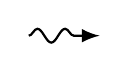
\begin{tikzpicture}
   \draw [decorate, decoration={snake}, black,  thick ] (0.1,0)--(0.8,0)  ;
   \draw [ black,  very thick,  -> , baseline, -latex] (0.8,0)--(1.0,0) ;
  \end{tikzpicture}
  }

  \usepackage[normalem]{ulem}

  \setlength{\parindent}{0cm}
  \setlength{\parskip}{0.4em}

  \titleformat{\section}
    {\normalfont\fontsize{12}{12}\bfseries}{\thesection}{1em}{}



  \usepackage{tabu}
  \usepackage{longtable}
  \usepackage[table]{xcolor}

  \definecolor{tableHeader}{RGB}{211, 47, 47}
  \definecolor{tableLineOne}{RGB}{245, 245, 245}
  \definecolor{tableLineTwo}{RGB}{224, 224, 224}

  \newcommand{\tableHeaderStyle}{
      \rowfont{\leavevmode\color{white}\bfseries}
      \rowcolor{tableHeader}
  }

\usepackage{multirow}
  \begin{document}
%%%%%%%%%%%%%%%%%%%%%%%%%%%%%%%%%%%%%%%%
\setcounter{page}{1}

\begin{center}
  \fontsize{12}{2em}
  \selectfont
  Understanding the origin of toughness enhancement in complex architectured ceramic composites by developing and using an anisotropic variational fracture theory
\end{center}
%%%%%%%%%%%%%%%%%%%%%%%%%%%%%%%%%%%%%%%%

%%%%%%%%%%%%%%%%%%%%%%%%%%%%%%%%%%%%%%%%%%%%%%%%%%%%%%%%%%%%%%
%%%%%%%%%%%%%%%%%%%%%%%%%%%%%%%%%%%%%%%%%%%%%%%%%%%%%%%%%%%%%%
%%%%%%%%%%%%%%%%%%%%%%%%%%%%%%%%%%%%%%%%%%%%%%%%%%%%%%%%%%%%%%
\section{Introduction}
  \label{s:Intro}

  %%%%%%%%%%%%%%%%%%%%%%%%%%%%%%%%%%%%%%%%%%%%%%%%%%%%%%%%%%%%%%
  \subsection{Research objective (\emph{Ro}):}
    \label{s:ro}
    \emph{We seek to understand how architectural motifs in 3D ceramic composites affect their toughness and damage tolerance. This will be done by developing a new variational fracture theory that can accurately simulate the evolution of complex crack topologies in ceramic composites, and predict their bulk mechanical responses from their architecture and material properties.}

    Ceramics are lighter than metals and are able to withstand higher temperatures and corrosive environments. This makes them appealing for aerospace, transportation, and energy production technologies \cite{padture2016advanced}. However, because they are brittle, ceramics are ill-suited for applications in which reliability is of paramount importance. To increase their toughness and damage tolerance, ceramics are often made into composites. The small-scale architecture of ceramic composites is known to be intimately connected to their large-scale toughness and damage tolerance \cite{clegg1990simple,meyers2013structural,kolednik2011bioinspired}. However, understanding how changes in a composite's architecture will affect these properties is currently an open challenge.

    Recently, techniques adopted from the textile industry \cite{padture2016advanced}, as well as new digital manufacturing processes \cite{minatto2015multilayered,karambelas2013strombus,barthelat2015architectured,corni2012review} have greatly expanded the diversity and complexity of ceramic composite architectures. With the possibility to fabricate an even wider range of complex, 3D architectures (see Figure \ref{f:intro} (c)), it is important to know which architectural motifs are most beneficial.

    Some structural biomaterials (SBs), such as bone and shell, are much tougher and more damage tolerant than their constituents because of their intricate architectures (see Figures \ref{f:intro} (a)--(b) and \ref{f:hyp} (c)) \cite{wegst2015bioinspired,kamat2000structural,barthelat2011toughness,currey2003well}. They therefore serve as a good starting point for determining which architectural motifs enhance toughness and damage tolerance. We propose to investigate the fundamental physics and mechanics that govern how small-scale architecture and heterogeneity connect to large-scale toughness in ceramic composites, like SBs.

    \begin{figure}[h!]
      \centering
        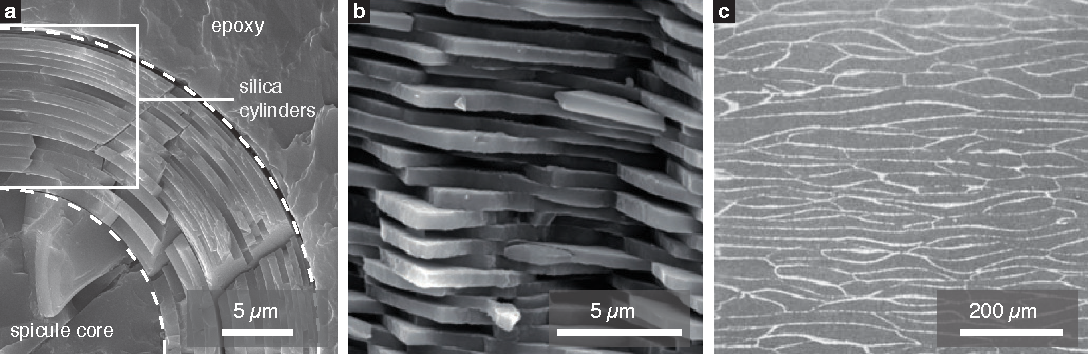
\includegraphics[width=\textwidth, trim={0 0.0cm 0.0cm 0}, clip]{Figures/Introduction/IntroFig_V6.pdf}
        \caption{ \footnotesize The complex architecture of SBs and ceramic composites. (a) Cylindrical, concentric layers of silica in the spicules of the marine sponge \textit{Euplectella aspergillum} (modified from \cite{monn2015new}). (b) Brick-and-mortar architecture of calcium carbonate tablets in nacre (molluscan shell) (reprinted from \cite{ritchie2011conflicts}). (c) A SiC/graphite composite made using fibrous monolith construction techniques (reprinted from \cite{baskaran1993fibrous}).
          }
        \label{f:intro}
    \end{figure}

  %%%%%%%%%%%%%%%%%%%%%%%%%%%%%%%%%%%%%%%%%%%%%%%%%%%%%%%%%%%%%%
  \subsection{Hypothesis underlying the proposed research}
       \label{s:hyp}
       We hypothesize that the toughness enhancement in composites with complex architectures is due to the interfaces within them acting as traps and mazes (see Figure \ref{f:hyp} (a)--(b)). The stiff phases fail through brittle fracture. However, the interfaces trap the cracks and make them consume much more energy to spread across the specimen. They do this primarily by pinning, deflecting, and splitting the cracks~\cite{gao1989first,dalmas2009crack,gu1997crack}. Our hypothesis is motivated by experimental observations of dense crack patterns in failed composites~\cite{barthelat2007experimental,poissant2010novel}, our preliminary results (see \S \ref{s:curr}), and the PI's previous research on contact interface toughening caused by surface architectures (see Section \S \ref{s:prev})~\cite{kesari2010role,kesari2011mechanics,kesariPML}.

       \begin{figure}[h!]
         \centering
           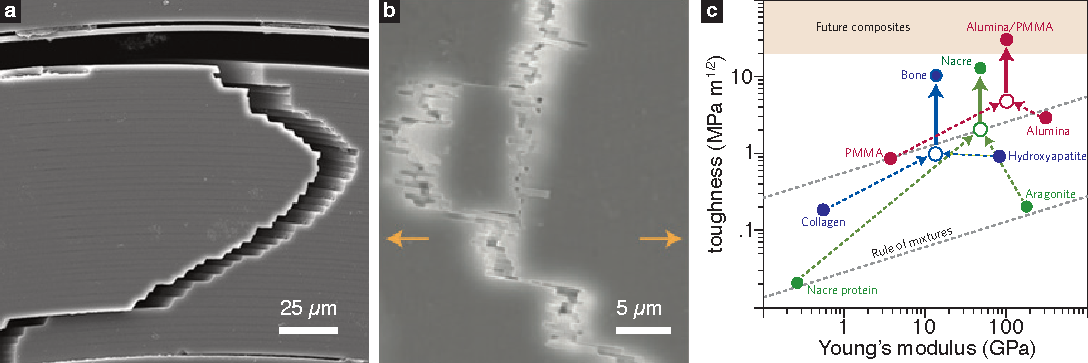
\includegraphics[width=\textwidth, trim={0 0.0cm 0.0cm 0}, clip]{Figures/Introduction/CrackPath_V2.pdf}
           \caption{ \footnotesize Complex crack paths in ceramic composites are responsible for toughness enhancement. (a) Cracks are deflected and split by the concentric layered architecture of a \textit{Monorhaphis Chuni} spicule (reprinted from \cite{Weaver:2010ew}). (b) Crack splitting and tablet pull-out observed during the fracture of nacre loaded in uniaxial tension (reprinted from \cite{wegst2015bioinspired}). (c) Comparison of toughness of both nacre and SB-inspired layered ceramic composites with their brittle constituents showing a toughness enhancement in excess of what is predicted by the rule of mixtures~(reprinted from \cite{wegst2015bioinspired}).
             }
           \label{f:hyp}
       \end{figure}

  %%%%%%%%%%%%%%%%%%%%%%%%%%%%%%%%%%%%%%%%%%%%%%%%%%%%%%%%%%%%%%
  \subsection{Novelty of the proposed research:}
    \label{s:nov}
    Applied mechanics models are often used to determine the optimal set of architectural parameters for enhancing toughness in composites. Due to the complexity of 3D composite and SB architectures, however, it is seldom clear which features and associated toughening mechanisms are important and should therefore be included in a model. Naturally, by focusing on different subsets of features one can come up with a number of models~\cite{barthelat2007mechanics,smith1999molecular,meyers2008mechanical,li2004nanoscale,lin2006mechanical,chen2013bio}. Since it is not possible to simply ``see'' inside the material and check whether the mechanisms presumed in the models are truly active, it is difficult to determine the validity of any of the models.

    Due to the complexity of their architectures, a mathematically robust computational framework is required to capture the nucleation and evolution of complex crack patterns in SBs and ceramic composites.

    \begin{figure}[h!]
      \centering
        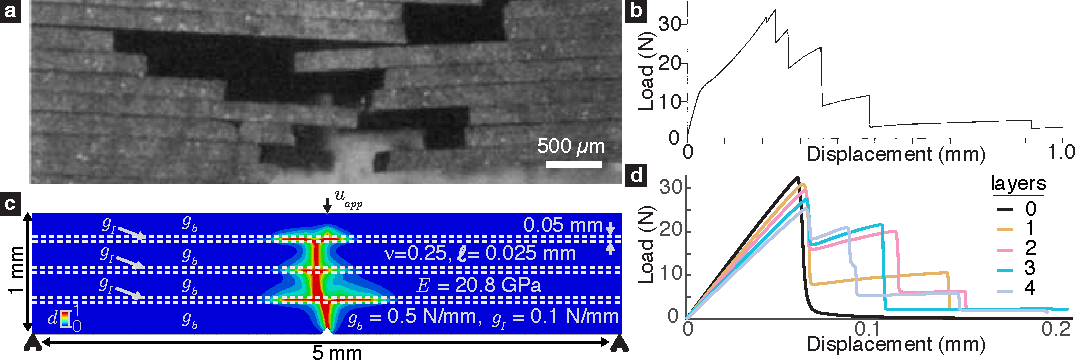
\includegraphics[width=\textwidth, trim={0 0.0cm 0.0cm 0}, clip]{Figures/Introduction/CrackPathSim_V1.pdf}
        \caption{ \footnotesize Initial RVFT results show accurate predictions of crack paths and capture toughening mechanisms such as crack deflection in 2D composites. (a) The convoluted crack path in a 2D layered SiC/graphite composite loaded in three point bending. (b) The load-displacement response of the SiC/graphite composite. (a), and (b) are reprinted from \cite{clegg1990simple}. (c) Crack path predicted by the RVFT tool for a model of the composite shown in (a). (d) The load-displacement response obtained from the RVFT tool predictions for different numbers of layers.
          }
        \label{f:sim}
    \end{figure}

    Conventional fracture simulation tools, such as element deletion methods~\cite{komori2001simulation,saanouni2004numerical}, singularity element methods~\cite{henshell1975crack,barsoum1977triangular,akin1976generation}, cohesive zone method (CZM)~\cite{needleman1987continuum,tan2007constitutive} and even extended finite element method (XFEM)~\cite{dolbow1999finite, stolarska2001modelling, belytschko2003dynamic,huang2003modeling} are not able to accurately capture the crack topology changes that occur in ceramic composites (see Table~\ref{t:comp}). In contrast, regularized variational fracture theory (RVFT) provides a straightforward way to simulate these highly complex crack patterns. The RVFT is an approximate model for fracture in which complex crack patterns are represented by the level set of a scalar-valued field called the damage field \cite{bourdin2000numerical}.

    \paragraph{Cohesive zone (CZ) methods} have proven to be very significant for modeling interfacial fracture. There are several versions of CZ methods discussed in literature. Most of those methods can be put into two primary classes. The first class is roughly based on the numeric implementation of Hillerborg et al.\cite{hillerborg1976analysis}  while the second class is based on the ideas of Xu and Needleman~\cite{xu1994numerical}, and Camacho and Ortiz \cite{camacho1996computational}. Both classes are based on the work of Dugdale \cite{dugdale1960yielding} and Barenblatt \cite{barenblatt1962mathematical} and built atop of classical finite elements technqiues. In that crack growth is modeled by allowing adjoining finite  element pairs to separate along their shared boundary. As the elements seperate, tractions are applied on the separating faces of the elements as per a pre-assigned traction-separation law. The shape and parameters in the traction separation law are chosen to model different types of damage behavior (ductile, quasi-brittle, etc.). This idea is made numerically feasible by incorporating what are termed \textit{cohesive zone (or interface) elements} between the shared boundaries of adjoning finite element pairs. The primary difference beween the two classes of CZ methods is in the selection of the finite element boundaries at which the CZ elements are included.

    In the classical version of the CZ method, given by Hillerborg et al., the CZ elements are only placed along finite element boundaries which are known\slash expected to be close to the final crack path. Thus, the application of the classical CZM is  predicated upon having some \textit{a priori} knowlege of the crack path. However, the success of the proposed research program hinges on developing and leveraging the ability to predict the evolution of complicated crack paths of which we have no or very little \textit{a priori knowledge}. Consequently, classical CZ methods are not suitable for the proposed research project.%√∏

    In the generalized version presented by Xu and Needleman the CZ elements are placed between all shared boundaries of the finite elements. This enables the simulation of crack propagation without requiring any \textit{a priori} knowledge of the crack path. This  generalized version is also capable of modeling the evolution of complicated crack paths. However, based on our study of the computational mechanics literature and the preliminary research that we undertook for planning the proposed project we found that the  generalized  CZ method is not very accurate in reproducing experimentally observed crack paths~\cite{tijssens2000numerical,de2003numerical,de2004computational}. For example,  Figure~\ref{f:czm} shows a comparison between  experimentally observed crack paths and those that were computationally predicted using the generalized CZ method. As can be seen by comparing Figure~\ref{f:czm}(a) with either (b) or (c),  the generalized CZ method predicted cracks paths are quite different from the experimentally observed ones.  Furthermore, as can be seen from Figs.~\ref{f:czm}(b)--(c), the generalized CZ method predicted crack paths are \textit{mesh dependent}. That is, they depend on the size and structure of the finite element mesh employed.

    The inaccuracy and  mesh sensitivity of the generalized CZ method is widely discussed in literature \cite{de2003numerical,de2004computational,tijssens2000numerical,song2008comparative}. For example, it is well known that  the crack path predicted by CZ method is inherently biased because crack growth in it is restricted to inter-finite element boundaries. This could give rise to mesh dependent crack paths. Also, Borst \cite{de2003numerical,de2004computational} gives the following reason for the method's poor performance. In theory, a CZ element is supposed to have infinite stiffness before the traction acting on it reaches a critical value, i.e, prior to initiation of any damage in it. In practice, however, in order to make the numerical implementation feasible, the CZ elements are provided with a finite stiffness  in the simulations. However, assigning a finite stiffness to the CZ elements can artifically change the bulk elastic constitutive behavior of the material composing the solid, since recall that the CZ elements are placed between all finite element boundaries in this method. This artifact can be avoided by increasing the CZ elements' stiffness. But that has the consequence of increasing the condition number of the numerical matrices in the simulation making the calculations unstable and prone to numerical errors. Borst suggests that this no win situation in selecting an ideal stiffness for the CZ elements coupled with the CZ elements being present between all shared finite element boundaries is the primary reason behind the method's poor performance.

    We do not have any ideas as how to remedy the generalized CZ method's poor accuracy and high mesh sensitivity. Therefore, we decided not to select it for further development for the purpose of our pursing the project's overarching research objective.

    \begin{figure}
          \centering
          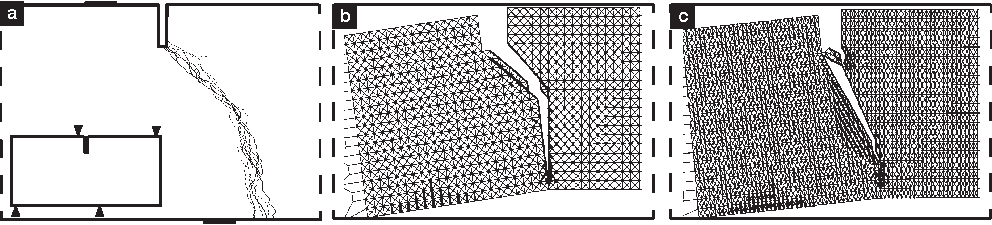
\includegraphics[width=1.0\textwidth]{Figures/CZM/CZM_crack_path_ver3.pdf}
          \caption{\footnotesize Comparison between experimentally observed and computationally predicted crack paths. (a) shows the experimental crack paths observed in concrete specimens by Schlangen~\cite{schlangen1993experimental} and the corresponding experimental setup is shown in the inset, which is a single edge notch (SEN) shear load test. Each curve corresponds to a different specimen. (b) and (c) show the computationally predicted crack paths for a coarse and fine finite  element mesh, respectively. These computational crack paths  were predicted by Tijssens\textit{et al.}~\cite{tijssens2000numerical} for the experiments shown in (a) using the generalized CZ method.}
          \label{f:czm}
    \end{figure}

    \begin{figure}
          \centering
          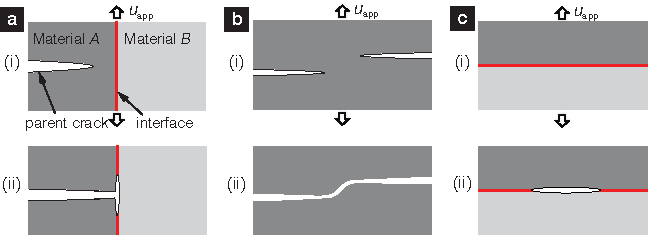
\includegraphics[width=1.0\textwidth]{Figures/CZM/CrackPathTopology_V1.pdf}
          \caption{\footnotesize}
          \label{f:topchanges}
    \end{figure}

    \paragraph{Extended Finite Element methods (XFEM).} The XFEM is a remarkable method. It has been used to  simulate quasi-static crack growth in both 2D~\cite{belytschko1999elastic,bordas2007extended,dolbow1999finite} and 3D~\cite{sukumar2000extended,moes2002non,gravouil2002non}, and dynamic crack growth in 2D~\cite{belytschko2003dynamic,song2006method}. It is currently widely used to predict crack paths~\cite{golewski2012numerical,barkai2012crack,peng2017extended} and is even a feature in the commercial finite element software package Abaqus~\cite{abaqus2014}. It was introduced by Belytschko and Black \cite{belytschko1999elastic} for modeling cracks in solids without the need for remeshing. The numerical ideas underlying XFEM  are based on the partition of unity concept of Melenk and Babu\v ska~\cite{melenk1996partition}.  Currently, there are several versions of the XFEM  discussed in its literature. So, it is not unlikely that our comments will not apply to all of them. Also, we have sincerely tried not to cherry pick which features of the XFEM we discuss so as not to give an unfair appraisal of its capabilities.

    Like CZ methods, the XFEM too is built atop of finite elements methods. In  standard finite element method (FEM), the displacements, strains, etc. are approximated as  linear combinations of a select set of functions called  the \textit{basis functions}. Choosing a finite element mesh and the finite element type(s) (linear tetrahedron, etc.) in a problem  is tantamount to choosing the set of basis functions. In standard FEMs, the basis functions are usually continuous or smooth. The coefficients of the basis functions in the linear combinations are related to the degrees of feedom at the finite element nodes. In simulations based on  standard FEMs, the set of basis functions remains fixed during the simulations. The ingenuity of the XFEM lies in the following two modifications: (i) In addition to the usual continuous/smooth basis functions, discontinuous and irregular basis functions are allowed in the  set of basis functions. This process is called \textit{enrichment}. The choice of these discontinuous/irregular basis functions is  based  on the asymptotic solutions of fracture problems in the linear theory of elasticity and the total deformation theory of plasticity. These new basis functions enable the XFEM to capture the discontinuties across the crack's faces and the singular behavior  at its  tip. (ii) The  crack growth is modeled by allowing the set of basis functions to change as the crack grows.

    Despite its tremedous utility,  the XFEM is not suitable for pursuing the objectives of the current porposal. This is  because  the XFEM in its classical form cannot  be used to  model topology changes (see, e.g., Figure~\ref{f:topchanges}). That is, it cannot  be used to capture phenomena such as  the merging of two (or more)  cracks to  form a single crack (Figure~\ref{f:topchanges}(a).i--ii), the splitting of a crack into two (or more)  daughter branches (Figure~\ref{f:topchanges}(b).i--iii), and  the nucleation of new cracks (Figure~\ref{f:topchanges}(c).i--iii).  This is not to say that XFEM cannot  apply to a crack that contains one of more branches. Indeed, special  enrichement functions have been developed through which  XFEM  can yield  the  displacements, stresses, etc.  in  problems that contain a crack with  multiple branches~\cite{daux2000arbitrary,belytschko2001arbitrary}. However, even  with those special enrichments  the XFEM  on its own---i.e., without any modeler input during the simulation, or \textit{a priori} knowledge about any  forthcoming topolology changes---will not be able to predict whether or not a  crack will split into mutiple branches, and if does split, how many branches it will split into.

    Topology changes are not very common in quasi-static crack growth problems in homogenous materials. However, as we discussed in \S XXX,  topology changes are very common in heterogenous materials, such  as structural biomaterials. In fact,  topology changes are a key feature of the  mechanisms  through which  hypothesize that the structural biomaterials  gain their remarkable   toughness. It is possible to augument the XFEM with features from CZ methods~\cite{wells2001new,moes2002extended,mariani2003extended}, or using older failure theories, such as the  \textit{critical principle stress failure criteria}, to give XFEMs some capability  for capturing toplology changes. However, we are not aware of any rational/scientific  theory that can guide such an augenmentation. Without a systematic means  to  guide the augumentation, we are afraid  that any such augementations can only be  hueristic or \textit{ad-hoc}  at best and therefore cannot be the primary agenda of a scientific project. The  RVF theory, on the other hand, can readily model topology  changes without any heuristic/\textit{ad-hoc} augumentations, see  Figure~\ref{f:xfem} and Figure~\ref{second figure}, e.g.   For these reasons, we decided not to select the XFEM for  pursuing  the  project's research objective.

    \begin{figure}[ht!]
      \centering
      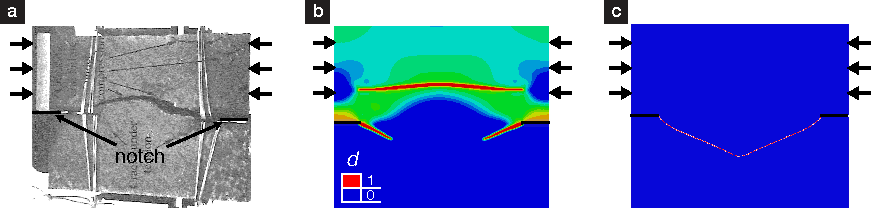
\includegraphics[width=\textwidth]{Figures/XFEM/concrete_ver2.pdf}
      \caption{Comparison between experimentally observed and computationally predicted crack paths. (a) shows a photograph of a failed concrete specimen. This is from the expeiments reported by G{\'a}lvez \textit{et al.}~\cite{galvez1999fracture}.   The specimen was prepared by  cutting two notches, one  on each of its   left and righ edges.  The only loading on the specimen was on its  top portion. That is,   the region above the notches was loaded in compression. The specimen was observed to fail through the formation and  propagation of two distinct crack systems.  The first system   (marked in red dashed lines)  consists  of a two cracks, each of which  emanate  from a  notch and  grow a short distance into the  bottom portion of the specimen. The second system (marked in yellow dash-dot lines) consists  of a single crack that nucleates in the top portion of the speciemen and propagates symmetrically towards the left and right.  (b) shows the predictions of the RVFT.  As can  seen, the    RVFT captures both system 1 and 2 of the cracks formed. Its predicted shape and length of the  system 1 cracks is also quite consistent with what is experimentally observed.  Its  predicted shape and length of the system 2 crack is  slightly different from what is observed in experiments. We believe that this disparity is due to the incomplete knowledge we have about the specimen's materials properties and the experiment's loading program. (c) shows the predictions from the XFEM (as implemented in Abaqus). The XFEM method is able to capture the system 1 cracks. However, it completely misses the  system 2 cracks. This is expected, since as we discuss in the text, XFEM on its own cannot readily capture  toplogy changes, of which crack nucleation is a special case. Also, the XFEM predicted length of the  system 1 cracks is substantially  different from what is observed experimentally. }
      \label{f:xfem}
\end{figure}

%
\taburowcolors[2] 2{tableLineOne .. tableLineTwo}
%\tabulinesep = ^4mm_3mm
\tabulinesep = ^2mm_1mm
\everyrow{\tabucline[.4mm  white]{}}

    %\begin{table}
\begin{tabu}{ X[c,3] X[c,3] X[c,4] X[c,3] X[c,4]  X[c,4] }
\tableHeaderStyle
      CZM (Hillerborg \textit{et al.}) & CZM (Xu and Needleman) & Damage mechanics &  Element Deletion  & XFEM  & RVFT \\
    \multicolumn{6}{p{0.97\textwidth}}{\textbf{\textit{No need of \textit{a priori} knowledge of crack path(s), i.e.,  capable of capturing topology changes without user input, or resorting to \textit{ad-hoc}, or heuristic techniques.}}}\\
           No\cite{hillerborg1976analysis} & Yes\cite{xu_1994,tijssens2000numerical}  & Yes\cite{peerlings1998gradient} & Yes & No\cite{belytschko2001arbitrary,daux2000arbitrary} & Yes\cite{borden2012phase} \\
           \multicolumn{6}{p{0.97\textwidth}}{\textbf{\textit{Good accuracy. That is, able to quantitatively reproduce experimental observations of growth of cracks and the evolution of a crack network as long as there are no  topology changes in the network .)}}}\\
          - &  No\cite{tijssens2000numerical,de2003numerical,de2004computational} & No  & No\cite{song2008comparative} & competitive & competitive \\
        \multicolumn{6}{p{0.97\textwidth}}{\textbf{\textit{Well conditioned, i.e., no problems with numerically stablility.}}}\\
          Yes & Yes & No & Yes &  No\cite{bechet2005improved} & Yes \\
          \multicolumn{6}{p{0.97\textwidth}}{\textbf{\textit{Mesh independence.}}}\\
           No & No\cite{tijssens2000numerical,de2003numerical} & No & No\cite{song2009cracking} & Yes\cite{nicOlas1999finite} & Yes\cite{miehe2010thermodynamically,bourdin2000numerical,borden2012phase} \\
        \multicolumn{6}{p{0.97\textwidth}}{\textbf{\textit{Computationally affordable.}}}\\
        Yes & Yes & No & Yes &  Yes & No\\
        \multicolumn{6}{p{0.97\textwidth}}{\textbf{Table. 1}: A comparison of different computational frcature mechanics methods, w.r.t. features that are critical  for pursuing the research objective}
\end{tabu}
    %     \caption{\footnotesize Comparison of computational fracture mechanics frameworks to evaluate features critical for pursuing the proposed research}
    %     \label{t:comp}
    % \end{table}






%         \begin{table}
%         \begin{tabu}{ X[l, 6] X[c,3] X[c,3] X[c,4] X[c,3] X[c,4]  X[c,4] }
% \tableHeaderStyle
%     Features critical in the computational tool for pursuing the research objective & CZM (Hillerborg \textit{et al.}) & CZM (Xu and Needleman) & Damage mechanics &  Element Deletion  & XFEM  & RVFT \\
%         No need of \textit{a priori} knowledge of crack path(s), i.e.,  capable of capturing topology changes without user input, or resorting to \textit{ad-hoc}, or heuristic techniques.  & No\cite{hillerborg1976analysis} & Yes\cite{xu_1994,tijssens2000numerical}  & Yes\cite{peerlings1998gradient} & Yes & No\cite{belytschko2001arbitrary,daux2000arbitrary} & Yes\cite{borden2012phase} \\
%         Good accuracy. That is, able to quantitatively reproduce experimental observations of crack paths and topology evolution. & - &  No\cite{tijssens2000numerical,de2003numerical,de2004computational} & No  & No\cite{song2008comparative} & competitive & competitive \\
%         Well conditioned, i.e., no problems with numerically stablility. & Yes & Yes & No & Yes &  No\cite{bechet2005improved} & Yes \\
%         Mesh independence. &  No & No\cite{tijssens2000numerical,de2003numerical} & No & No\cite{song2009cracking} & Yes\cite{nicOlas1999finite} & Yes\cite{miehe2010thermodynamically,bourdin2000numerical,borden2012phase} \\
%         \multicolumn{6}{c}{Multi-column}\\
%         Computationally affordable. & Yes & Yes & No & Yes &  Yes & No\\

%     \end{tabu}
%         \caption{\footnotesize Comparison of computational fracture mechanics frameworks to evaluate features critical for pursuing the proposed research}
%         \label{t:comp}
%     \end{table}{}

    If the RVFT is to function as an investigative tool for identifying the key architectural features, then it is important that it is able to reproduce the salient features of the experimentally observed failure responses of composites (see Figure \ref{f:sim}). However, the current RVFT was formulated with a minimal inclusion of mechanics and physics principles. For that reason, in many instances, RVFT predicts unphysical behaviors. For example, cracks in RVFT have finite thickness.  This contrasts with the conventional description of a crack as having zero thickness. It, however, does not preclude RVFT from  producing accurate predictions as long as the crack thickness remains small and does not broaden as the crack grows (see \S \ref{s:curr} and Figure \ref{f:VFTvalidation}). In the current RVFT formulation, this crack broadening can be controlled or limited to some extent at the expense of computational complexity.

    However, the required increase in computational expense makes the RVFT untenable for performing the large parametric studies required to understand the connection between architecture and toughness in composites. We believe this ``crack broadening'' problem is the most important of the unphysical behaviors of the current RVFT that prevents it from being used as a way to investigate toughness enhancement in composites (see \S \ref{s:propres}). The new RVFT that we propose uses a strategy that we have developed to completely eliminate the problem of crack broadening. We refer to our new RVFT as anisotropic RVFT (aRVFT) and describe our strategy in detail in \S \ref{s:propres} and \ref{s:A1}. By eliminating this fundamental problem, our simulations will not only be much less computationally expensive, and therefore able to simulate fracture in composites with complex, 3D architectures, but they will also be more physically realistic.

%%%%%%%%%%%%%%%%%%%%%%%%%%%%%%%%%%%%%%%%
%%%%%%%%%%%%%%%%%%%%%%%%%%%%%%%%%%%%%%%%
%%%%%%%%%%%%%%%%%%%%%%%%%%%%%%%%%%%%%%%%
\section{Previous and current work that motivates our hypothesis}
  \label{s:prevcurr}

  %%%%%%%%%%%%%%%%%%%%%%%%%%%%%%%%%%%%%%%%
  \subsection{Previous work}
    \label{s:prev}
    Wavy interfaces are a prominent architectural motif in architectured SBs, such as woodpecker beaks (see Figure~\ref{f:VFTprelimresults}~(a)) and the cranial bones of rams, that are subjected to impact or cyclic loads but must remain intact to perform their mechanical functions \cite{lee2014hierarchical, jaslow1990mechanical}.

    In experiments that involve contact with adhesion between two surfaces, two distinct contact force ($P$) versus indentation depth ($h$) curves are often found depending on whether the indenter moves towards or away from the sample (see Figure~\ref{f:contact} (a)).
    %
    Moreover, the hysteretic energy loss is observed to depend on the maximum indentation depth (marked $|h_{\rm min}|$ in Figure~\ref{f:contact} (a)) in a load-unload cycle.
    %
    The PI's experiments \cite{kesari2010role} and continuum mechanics based theoretical work \cite{kesari2011effective} showed that the hysteresis can exist without moisture, plasticity, or viscoelasticity and that its magnitude depends on surface roughness.
    %
    The continuum mechanics models involved approximating the surface roughness with axisymmetric waviness of wavelength $\lambda$.
    %
    As seen in Figure~\ref{f:contact} (b), the surface waviness can create many metastable states for the contact interface at each value of the loading parameter $h$.
    %
    The hysteresis results from the fact that the system visits the state with the smallest contact size during the loading stage and the state with the largest contact size during the unloading stage (Figure~\ref{f:contact} (b)).
    %
    The energy loss is the result of a series of surface instabilities (marked with dashed magenta lines in Figure~\ref{f:contact} (b)), in which the contact area grows or recedes by a finite amount.
    %
    As $|h_{\rm min}|$ increases, so do the number of instabilities and hence the energy loss.
    %
    Studying the asymptotic behavior of the continuum theory in the limit $\lambda \to 0$(Figure~\ref{f:contact} (b)--(c)), it was found that the ($h$, $P$) points measured in an experiment would satisfy the equations
    %
    \begin{subequations}
    \label{eq:P-h}
    \begin{align}
    P(a) &= \frac{4E^*}{3R}a^3 - \sqrt{8\pi w E^*} a^{3/2} \pm 2\pi E^* A \lambda^{1/2} a^{3/2}, \label{eq:P}\\
    h(a) &= \frac{1}{R}a^2 - \sqrt{\frac{2\pi w}{E^*}}a^{1/2} \pm \pi A \lambda^{1/2} a^{1/2}, \label{eq:h}
    \end{align}
    \end{subequations}
    %
    where $a$ is the contact radius, $E^*$ the plane strain Young's modulus, $A$ is the amplitude of the surface
    waviness, and $R$ is the radius of the spherical indenter.
    %
    The $+$ and $-$ signs correspond to the loading and unloading stages of the experiment, respectively.
    %
    The Eqs.~\eqref{eq:P}--\eqref{eq:h} reveal that even though the intrinsic work of adhesion, $w$, remains constant, the experiments measure a higher effective work of adhesion of $w_{\rm eff}^{1/2} = w^{1/2} + A(\pi E^* \lambda/2)^{1/2}$ during the loading state and a lower value of $w_{\rm eff}^{1/2} = w^{1/2} - A(\pi E^* \lambda/2)^{1/2}$ during the unloading state.
    %
    %
    % \begin{figure}[h]
    %   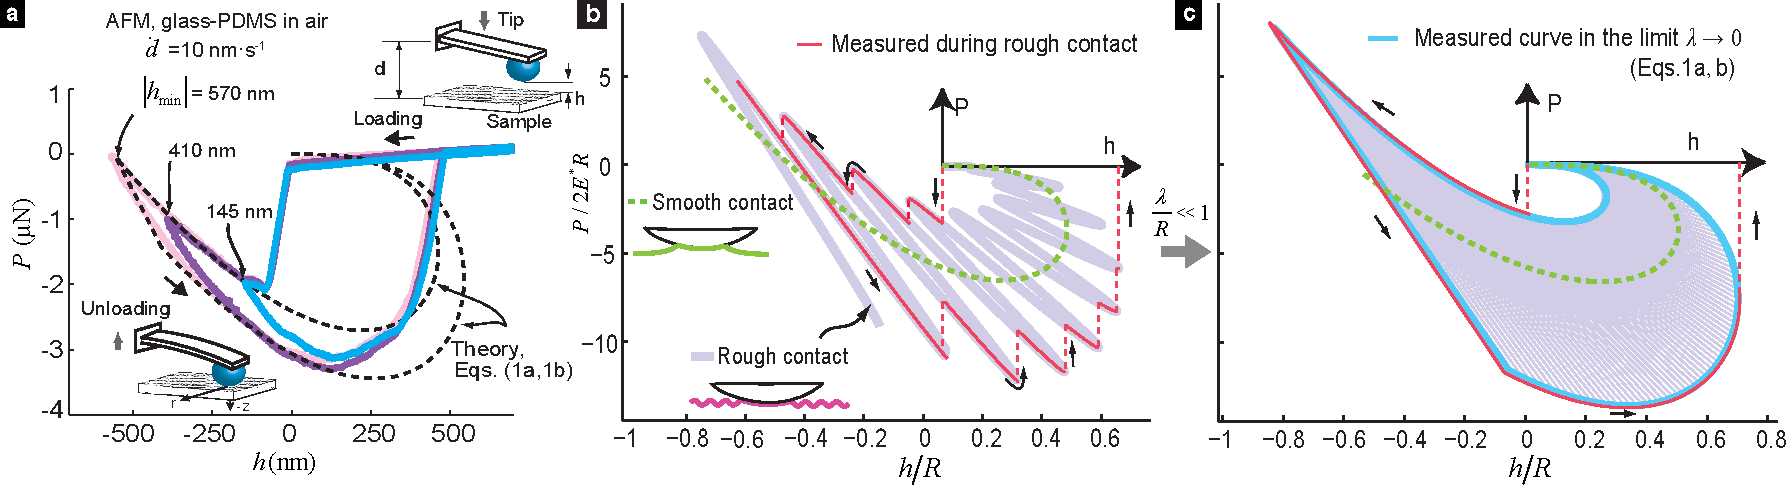
\includegraphics[width=\textwidth]{../../Proposal/ProjectDescription/Figures/WavyInterface/DDHAFM.pdf}
    %   \centering
    %   \caption{\footnotesize (a) The contact force $P$ as a function of indentation depth $h$ (shown marked in (a)) during contact of glass and PDMS in air at an indenting rate of $\dot{d}$ = 10 nm/s, (b) the $P$--$h$ curves predicted by a smooth-surface contact model and by wavy-surface (``rough'') contact model, and (c) the measured $P$--$h$ curve described by Eqs.~\eqref{eq:P}--\eqref{eq:h} that are derived by studying the asymptotic behavior of wavy-surface contact model in the limit of $\lambda \to 0$ (figure adapted from \cite{kesariPML}).}
    %   \label{f:contact}
    % \end{figure}

    Therefore, based on his previous studies of adhesion between wavy surfaces, the PI believes that the wavy interfaces could be a key ingredient for enhancing the toughness of these materials \cite{li2012numerical,wang2012specific,zavattieri2007determination,haghpanah2014adhesively}.
    %
    Even though the interface's intrinsic adhesion energy is constant, the interface's waviness can increase the measured --- i.e., the effective --- adhesion energy.
    %
    Similar adhesion energy enhancement has been reported for thin films with adhesive heterogeneities~\cite{xia2015adhesion}.
    %
    Motivated by this discovery and the similarities between the mechanics of contact and fracture, the PI searched for new toughening mechanisms in materials with wavy interfaces.

  %%%%%%%%%%%%%%%%%%%%%%%%%%%%%%%%%%%%%%%%
  \subsection{Current work}
    \label{s:curr}
    One of the primary differences between the wavy surface adhesion and wavy interface fracture problems is that in the case of fracture, a crack is not required to travel along the interface as it is in the adhesion problem.
   %
   Rather, in the fracture problem, the crack can either travel along the interface or propagate through the bulk (see Figure~\ref{f:VFTprelimresults}~(c)). The RVFT tool is ideally suited to handle this additional level of complexity.

    As preliminary research, we implemented non-linear finite element techniques~\cite{belytschko2013nonlinear} to
    numerically solve the RVFT Eqns.~\eqref{eq:GE} using the algorithms presented in \cite{borden2012phase}.
    %
    The results of these calculations are shown in Figures~\ref{f:VFTvalidation}--\ref{f:VFTprelimresults}.
    %
    These results were generated for the special case of small deformations and $\Psi_0$ corresponding to the strain energy density of a homogeneous, isotropic, linear elastic material model.
    %
    We found that in many important cases the results of the RVFT match the predictions of linear elastic fracture mechanics (LEFM), see, e.g.,  Figure~\ref{f:VFTvalidation} (a).
    %
    It has also been shown that the crack path predicted by the RVFT matches the crack path seen in many experiments~\cite{miehe2010phase,borden2012phase,dally2015phase}.
    %
    We were also able to reproduce these results, e.g., see Figure~\ref{f:VFTvalidation} (b).

    \begin{figure}[t!]
      \centering
      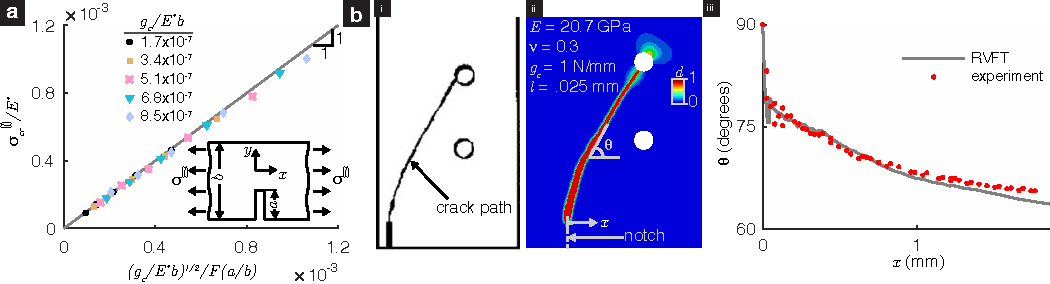
\includegraphics[width=\textwidth]{Figures/VRF/Figure1_box_ver9.pdf}
      \caption{\footnotesize Comparison of RVFT predictions with LEFM and experiments. (a) Edge-notched geometry subjected to a far-field stress $\sigma^\infty$. The dimensionless stress at which the crack initiates $\sigma^\infty_{cr}/E^*$ as a function of dimensionless variables, $g_c/E^*b$ and $a/b$ obtained from the analytical solution. For different values of $g_c/E^*b$, the markers lie close to the reference line shown in gray within an error of $5\%$. (b) Comparison of RVFT predictions with an edge notch three-point bending test in which the sample has three holes drilled in it. (i) The experimentally measured crack path from~\cite{bittencourt_1996}. (ii) Contour of the damage field $d$, where $d=1$ is indicated by red contour level signifying the location of the crack. (iii) Comparison of the measured crack path and the RVFT predictions using the crack angle, $\theta$ shown in (ii).}
      \label{f:VFTvalidation}
    \end{figure}

                    \begin{mdframed}
                       \paragraph{Technical details of RVFT}
                       Different versions of RVFT can be found in literature~\cite{bourdin_2008,hakim_2009}.
                       %
                       In our work we will focus on the RVFT presented by Bourdin et al.~\cite{bourdin2000numerical, bourdin_2008}.
                       %
                       In the last three years we have experimented with different RVFTs and found that Bourdin et al.'s is the most suitable for analyzing engineering problems, since it can be generalized and extended in a straightforward manner to handle finite deformations, dynamics, different hyperelastic material models, and complicated geometries and loading programs. Furthermore, Bourdin et al.'s theory has a  strong mathematical foundation.
                       %
                       The theory's underlying mathematical results make it clear as to what physics the theory is aiming to approximate, and give a rigorous proof, using the notion of $\mathit \Gamma$-convergence~\cite{braides2002gamma},  that the predictions of the theory will correctly capture that physics~\cite{chambolle_2005, ambrosio_1990b}.

                       The physics underlying Bourdin et al.'s RVFT is the variational fracture theory (VFT) put forward by Marigio and Francfort~\cite{francfort_1998}, which is a generalization of the configurational force balance ideas put forward by Griffith~\cite{griffith1921phenomena}. Griffith postulated that for a crack to grow the energy release rate should be equal to or exceed the fracture toughness of the material. The VFT generalizes this idea by postulating that on the application of a load increment, the observed crack pattern is the one which minimizes the total energy of the system over all admissible crack patterns. The admissible crack patterns are defined to be those that contain the crack pattern from the previous load increment as a subset. This constraint introduces irreversibility and history dependence into the problem.

                       In the absence of body forces, the total energy, $E$, can be written as the surface energy and what we define to be the equilibrium strain energy. The surface energy is  $\int_{\Gamma}g_c\, d\Gamma$,  where $\Gamma$ is the crack pattern and $g_c$ is the material's fracture toughness.
                       %
                       The strain energy  for a hyperelastic solid can be written as $\int_{\mathcal{B}_0\backslash \Gamma}\Psi_{0}(\bs{X}, \bs{C})\, d\Omega$, where $\Psi_0$ is the strain energy density, and $\bs{X}$ is a material point in the solid's reference configuration $\mathcal{B}_0$. The tensor $\bs{C}:=\bs{F}^{\rm T}\bs{F}$ is the right Cauchy-Green deformation tensor, where $\bs{F}=\bs{\nabla}_{0}\bs{u}+\bs{I}$ is the deformation gradient, $\bs{u}$ is the displacement vector, $\bs{I}$ is the identity tensor, and $\bs{\nabla}_0(\cdot)$ is the gradient operator defined with respect to $\bs{X}$. The equilibrium strain energy is then defined as the infimum value of the strain energy computed over the set of all admissible displacement fields. Note that the equilibrium strain energy term is a volume (resp. area) integral, whereas the surface energy term is a surface (resp. line) integral in 3D (resp. 2D). This makes it very difficult to solve the variational problem of finding the new crack pattern that minimizes the total energy after a load increment. To circumvent this problem,  Bourdin et al.~\cite{bourdin2000numerical} introduced the following regularized or ``smoothed'' energy functional,
                       %
                       \begin{equation}
                       \label{eq:PFT-Functional}
                       E_{\ell}(\bs{u},d):=
                       \int_{\mathcal{B}_0}
                       \Psi_{d}(\mathbf{X},\bs{C}, d)
                       %g(d(\bs{X}))\Psi_{0}(\bs{C},\bs{X})
                       \, d\Omega+
                       g_c/2
                       \int_{\mathcal{B}_0}
                       \left(
                       d(\bs{X})^2/\ell + \ell \lVert\bs{\nabla}_0d(\bs{X})\rVert^2
                       \right)
                       d\Omega,
                       \end{equation}
                       %
                       where $\|\cdot\|$ is the Euclidean 2-norm, the parameter $\ell$ has units of length and is called the regularization parameter, $\Psi_{d}(\mathbf{X},\bs{C}, d)=(1-d)^2 \Psi_{0}(\bs{X}, \bs{C})$ is called the degraded strain energy density, and we call $d(\bs{X})$ the damage field, which takes values between zero and unity. By construction, as $d$ increases the material's capacity to store elastic energy degrades. Therefore, $d$ can be interpreted as a measure of damage. When $d=0$ the material point is completely undamaged, and when $d=1$ the material point has lost all capacity to store strain energy. The crack pattern region, $\Omega_c$, is now defined to be a path connected subset of the solid $\mathcal{B}_0$ such that $d(\bs{X})\ge c,~\forall\bs{X}\in \Omega_c$, where $c$ is a real number just smaller than unity, and the set $\{\bs{x}\in \Omega_c~:~d(\bs{X})=1\}$ is non-empty. Since all integrals in the functional $E_{\ell}$ are now over $\mathcal{B}_0$, we can attempt to minimize $E_{\ell}$ with respect to $(\bs{u},d)$ by solving its corresponding Euler-Lagrange equations (for details see~\cite{borden2012phase}).

                       If $(\bs{u}^*_{\ell},d^*_{\ell})$ are smooth minimizers of $E_{\ell}$ then it is necessary that they satisfy the Euler-Lagrange equations corresponding to $E_{\ell}$, which are,
                       %
                       \begin{equation}
                         \label{eq:GE}
                       \bs{\nabla}_0\cdot\bs{P}=0,
                       \qquad\text{and}\qquad
                       g_c\ell\bs{\nabla}_0 \cdot (\bs{\nabla}_0 d)-g_c d/l=\partial \Psi_d/\partial d,
                       \end{equation}
                       %
                       for all $\bs{X}\in \mathcal{B}_0$, where $\bs{P}$ is the first Piola-Kirchhoff stress tensor, which in the present case comes out to be equal to $(1-d)^2\partial \Psi_0/\partial \bs{F}$. The governing equations, Eqns.~\eqref{eq:GE}, are solved along with the standard displacement and traction boundary conditions, and the new boundary condition that the component of $\bs{\nabla}_0 d$ normal to the solid's boundary vanish. For ease of elaboration, in deriving Eqns.~\eqref{eq:GE}  we ignored the irreversibility/history-dependence constraint. See~\cite{miehe2010phase} for a version of the governing equations for $(\bs{u},d)$ that respects the irreversibility constraint.
                       %
                       As per the aforementioned $\mathit{\Gamma}$-convergence result, the crack region $\Omega_c^*$ that corresponds to the minimizer $(\bs{u}^*_{\ell},d^*_{\ell})$ converges to the crack path postulated by the VFT as $\ell \to 0$.
                    \end{mdframed}

    The PI then performed a preliminary study of crack propagation in materials with wavy interfaces using the RVFT tool (see Figure~\ref{f:VFTprelimresults}~(b)--(e)).
    %
    In these simulations we allowed $g_c$ to vary spatially, so that in most of the solid it had a high value, $g_{b}$, and at a predefined wavy interface of finite thickness, it had a low value, $g_{I}$.
    %
    In our preliminary simulations depending on the parameters $A/\lambda$ and $g_{I}/g_{b}$ the failure of the interface displayed very rich mechanics.
    %
    Here, $A$ and $\lambda$ are the amplitude and the wavelength of the interface, respectively.
    %
    For example, we found that at small $A/\lambda$ the crack always propagated  along the interface (see Figure~\ref{f:VFTprelimresults}~(c)).
    %
    However, at larger $A/\lambda$ the crack repeatedly ventured out of the interface into the bulk and then back into the interface through a series of energy dissipating instabilities, see Figure~\ref{f:VFTprelimresults}~(c).
    %
    The instabilities occurring during the crack propagation are identified and shown in Figure~\ref{f:VFTprelimresults}~(d)--(e).
    %
    This led to substantial toughening in the load-displacement response---i.e., area under the load-displacement curve (see Figure~\ref{f:VFTprelimresults}~(b)).
    %
    Namely, the peak load is increased by 6.8\% and the fracture toughness is enhanced by 55.3\%.
    %
    %
    \begin{figure}[h]
      \includegraphics[width=\textwidth,trim={0 4.8cm 0 0},clip]{../../Proposal/ProjectDescription/Figures/WavyInterface//SinusoidalInterfaceFigCrackPropagation_V7.pdf}
      \centering
      \caption{ \footnotesize (a) Wavy interfaces between keratin scales in the beak of the red bellied woodpecker (photo from \cite{birdpicture1}, micrograph reprinted from \cite{lee2014hierarchical}). (b) Load--displacement curves for different aspect ratios $A/\lambda$ of the interface shown in (c). (c) Crack propagation along a wavy interface for $A/\lambda = 0.16$ and 1, respectively. The interface is shown as a dashed line. (d) Zoom-in view of the load-displacement curve indicated by dashed circle in (b) showing the instabilities during the crack propagation. (e) Snapshots at instability points as indicated in (d).
      }
      \label{f:VFTprelimresults}
    \end{figure}

    These examples reveal two interface toughening mechanisms: instabilities induced by the unstable crack propagation through bulk material, and the nucleation of daughter crack ahead of the primary crack. These mechanisms cannot be captured by the CZM and XFEM simulations. The preliminary results suggest that the RVFM is a powerful approach through which we can investigate toughening mechanisms in materials with complex, 3D interfaces.

%%%%%%%%%%%%%%%%%%%%%%%%%%%%%%%%%%%%%%%%%%%%%%%%%%%%%%%%%%%%%%
%%%%%%%%%%%%%%%%%%%%%%%%%%%%%%%%%%%%%%%%%%%%%%%%%%%%%%%%%%%%%%
%%%%%%%%%%%%%%%%%%%%%%%%%%%%%%%%%%%%%%%%%%%%%%%%%%%%%%%%%%%%%%
\section{Proposed research}
  \label{s:propres}
  \textit{Problem statement:}
    A  crack by definition has zero thickness.
    %
    Almost all  continuum mechanics fracture theories model cracks as curves or  surfaces in the reference configuration.
    %, i.e., as having zero thickness.
    %
    Similarly,  some of the most important computational fracture mechanics models, such as XFEM and CZM, also model the cracks as having zero thickness~\cite{day1994zero,benvenuti2008regularized}.
    %
    In contrast, a very conspicuous feature of the RVFT is that in it the crack thickness is non-zero. Recall from~\S\ref{s:curr} that in RVFT the crack is defined as the region $\Omega_c$, which has the same dimensionality as the solid $\mathcal{B}_0$.
    %

    The fact that the crack thickness is non-zero in RVFT does not preclude RVFT from being a useful and predictive theory of fracture.
    %
    For instance, consider again the remarkable match of the RVFT's predictions with LEFM and experimental results shown in Figure~\ref{f:VFTvalidation}.
    %
    However, for the cracks in the RVFT theory to be  physically meaningful it is critical that their thicknesses be much smaller that the physical dimensions of the solid.
    %
    This is because in the RVFT the crack region $\Omega_{c}$ has zero stiffness.
    %
    Thus, if a crack thickness is not much smaller than the solid's dimensions then the situation resembles that of a solid undergoing plastic failure rather that brittle fracture.
    %
    It is generally argued that the thickness of the crack is of the of order  $\ell$, the regularization parameter~\cite{amiri2014phase}.
    %
    And hence by choosing $\ell$ to be much smaller than the characteristic dimension of the solid, $W$, i.e., $\ell/W\ll 1$, one can ensure that the results are always meaningful, i.e., the failure has the physical features of  brittle fracture.
    %
    However, in some test cases we observed that the crack thickness was comparable to the dimensions of the solid even though $\ell$ was much smaller than the solid's dimensions.
    %
    We termed this effect \textit{broadening}.
    %
    Example test cases displaying broadening are shown in  Figure~\ref{f:broadening}.
    %

    \begin{figure}[t!]
      \centering
        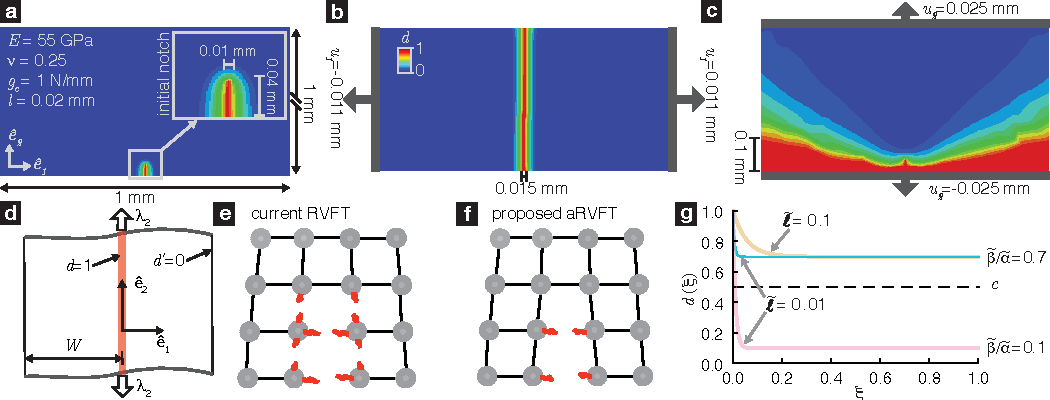
\includegraphics[width=\textwidth]{Figures/Broadening/Broadening_V9.pdf}
          \caption{ \footnotesize Example simulations demonstrating the problem of crack broadening. (a) Experiment geometry and problem parameters. Only the lower half of the plate in the $\hat{\mathbf{e}}_2$ direction is shown since $d\approx 0$ in the upper half for (a)--(c). The notch is not explicitly incorporated as part of the plate's geometry but rather is represented as a small region where $d=1$, as shown in the inset. (b) The plate in (a) is loaded in uniaxial tension by displacing the boundaries marked in gray in the $\pm \hat{\mathbf{e}}_1$ direction. A crack (the red contour level) propagates from the notch in the $\hat{\mathbf{e}}_2$ direction until the plate is cleaved into two pieces. The crack's thickness is roughly equal to $\ell$. (c) The plate in (a) is loaded in uniaxial tension parallel to the notch direction by displacing the boundaries marked in gray in the $\pm \hat{\mathbf{e}}_2$ direction. Damage progresses from the notch in the $\pm \hat{\mathbf{e}}_1$ directions until there is a region of completely disintegrated material (i.e., $d\approx1$) spanning the entire width of the plate. The thickness of this region is much larger than $\ell$. (d) A 2D strip with infinite length in the $\hat{\mathbf{e}}_2$ direction stretched parallel to a crack (shown in red) along its length. (g) The variation of the damage, $d$, over the half-width of the 2D cracked strip shown in (d). The variable $\xi=x/W$, and $x$ is the Cartesian coordinate in the  $\hat{\mathbf{e}}_1$ direction shown in (d).
      }
      \label{f:broadening}
    \end{figure}

    We found that the broadening effect was not due to human errors or numerical artifacts, but due to the inadequacy of the condition $\ell/W \ll 1$.
    %
    This  fact is best illustrated by the following analytical solution to the governing Eqns.~\eqref{eq:GE} for a simple boundary value problem.

    Consider a 2D strip of infinite length and width $2W$ that is shown in Figure~\ref{f:broadening} (d).
    %
    The strip is composed of an incompressible neo-Hookean material so that the degraded strain energy density in this case is $(1-d)^2 (\mu/2)(\lambda_1^2+\lambda_2^2-2)$.
    %
    The strip has a pre-existing crack along its length (shown in red in Figure~\ref{f:broadening} (d)).
    %
    Starting from this state, the strip is uniformly stretched with a stretch ratio of $\lambda_2$ in the crack direction (marked as $\hat{\mathbf{e}}_2$ in Figure~\ref{f:broadening} (d)).
    %
    Let  $\tilde{\beta}:= \mu (\lambda_2^2+1/\lambda_2^2-2) W^2 /g_c  \ell$ be a dimensionless measure of this straining, where $\mu$ is the shear modulus, and let $\tilde{\alpha}:=\tilde{\beta}+1/\tilde{\ell}^{2}$, where $\tilde{\ell}:=\ell/W$.
    %
    Assuming that the solution does not vary along the strip's length, an analytical solution for the damage field can be obtained for this problem.
    %
    It can be shown using the analytical solution that in the majority of the strip the damage variable is approximately equal to $ \tilde{\beta}/\tilde{\alpha}$, see Figure~\ref{f:broadening} (g).
    %
    If $ \tilde{\beta}/\tilde{\alpha}$ becomes greater than $c$, which, recall, is the parameter used for defining the crack region $\Omega_c$, then the crack width will become equal to the strip's width. That is, there will be broadening. And this would occur irrespective of how small $\tilde{\ell}$ is as long as $ \tilde{\beta}/\tilde{\alpha}$ is greater than $c$, see Figure~\ref{f:broadening} (g).
    %
    Therefore in order to prevent broadening, it is also necessary that $\tilde{\beta}/\tilde{\alpha}$ is much smaller than unity, which in terms of dimensional variables reads $\ell \ll \ell_c$, where $\ell_c:=g_c/\mu (\lambda_2^2+1/\lambda_2^2-2)$ is a length scale characteristic of the material and loading.
    %
    In summary, when the material and the loading are such that $\ell_c\ll W$, the condition $\ell \ll W$ alone is not sufficient to prevent broadening.

    Our preliminary research also has the following important consequence.
    %
    In view of broadening, current RVFT cannot be used as the basis for developing practical investigative tools.
    %
    As per the $\mathit{\Gamma}$ convergence proof mentioned in~\S\ref{s:curr} the solution to the Eqns.~\eqref{eq:GE} becomes meaningful only in the limit $\ell\to 0$.
    %
    From a practical perspective, the computational cost grows inversely with $\ell$.
    %
    Therefore, one would like to use as large an $\ell$ as possible.
    %
    However, the proof does not tell us what the largest value for $\ell$ is at which the results can still be meaningful.
    %
    Our analysis answers this question by stating that $\ell$ should at least be smaller than $\rm{min}\{W, \ell_c\}$.
    %
    This might suggest that the solution to the broadening problem is straightforward---simply make $\ell$ smaller than both $W$ and $\ell_c$.
    %
    However, this is much easier said than done.
    %
    For most practical applications, the value for $\ell_c$ is so small that using $\ell$ values smaller than $\ell_c$ is impractical.
    %
    For example, $\ell_c\approx 10\unit{nm}$ for silicon.
    %
    In 2D, even a $1\unit{\mu m}$ square specimen would require us solving one million equations.  Of course, with recent advances in parallelization and computational power it is routinely possible to solve such large systems of equations on computer clusters.
    %
    However, recall that the PI's scientific vision involves using RVFT computations as investigative tools.
    %
    This requires the analyst to run a RVFT simulation repeatedly to study the effect of different architectural features on the manner in which the crack patterns evolve and affect the toughness.
    %
    Currently, solving 0.3 million equations takes us 56 hours of CPU time when solving them in parallel on 16 CPU cores.
    %
    Thus, in summary, our analysis shows that broadening is a major problem, and because of it computational simulations based on the current RVFT cannot be used as practical investigative tools.

  %%%%%%%%%%%%%%%%%%%%%%%%%%%%%%%%%%%%%%%%%%%%%%%%%%%%%%%%%%%%%%
  \subsection{Research plan: aims and tasks}
    \label{s:aims}
    The overarching objective of the project is to investigate the connection between architecture and toughness in ceramic composites by testing the validity of our hypothesis (see \S \ref{s:hyp}). We split this primary objective into two parts: (\emph{Ro.1}) Developing a new variational fracture theory and computational framework that are capable of robustly simulating crack topology changes (crack branching, merging, etc.) in composites with complex, 3D architectures and heterogeneities, and (\emph{Ro.2}) Evaluating the predictive potential of the new theory by comparing its predictions with experiments. We will accomplish \emph{Ro.1} and \emph{Ro.2} by pursuing the aims A1 and A2 and by carrying out their associated tasks.

    \begin{description}
      \item[Aim 1 (A1):] Develop a new RVFT that will be free of the problem of crack broadening. XXX
      \begin{description}
        \item[Task A1.T1] \textit{XXX}
        \item[Task A1.T2] \textit{XXX}
      \end{description}

      \item[Aim 2 (A2):] If the new RVFT is to function as an investigative tool for identifying the key architectural features, then it is important that it is able to reproduce the salient features of the experimentally observed failure responses of composites. We will use a computational implementation of the new RVFT to simulate the failure of a model SB---spicules from the marine sponge \textit{Euplectella aspergillum}. We will then compare the results from the RVFT simulation with measurements from fracture tests conducted on the spicules and evaluate whether the RVFT was able to capture the spicules' failure behavior.
      \begin{description}
        \item[Task A2.T1] \textit{Build an aRVFT computational model for the spicule}. In order to build an aRVFT model of a spicule we must first characterize the spicule's architecture and measure the mechanical properties of its constituent material and the interfaces within it.
        \item[Task A2.T2] \textit{Characterize the spicules' failure behavior}. Perform three point bending tests on notched spicules and measure their load-displacement responses.
        \item[Task A2.T3] \textit{Compare the measurements to the aRVFT tool's predictions}. Use the load-displacement responses as well as the work of fracture, or the total energy dissipated during failure, as metrics for comparison.
      \end{description}
    \end{description}

    %\paragraph{Research products:}
      %We envision the computational tool based on aRVFT being used in the following way. Consider a composite that displays exceptional toughness in a fracture test. We would begin by building a family of computer aided design (CAD) models that incorporate different subsets of the composite's architectural features. We would then perform virtual mechanical tests on those CAD models using the aRVFT tools. Small-scale material parameters, such as interface toughness and strength, that are difficult to measure experimentally will be used as fitting parameters in the aRVFT computations to get their predictions to match the measurements as closely as possible. These predictions will be used to identify the smallest subset of architectural features that are responsible for the majority of the SB's toughness.  An applied mechanics model will then be built by incorporating only that smallest subset. The virtual tests will be further analyzed to identify the key mechanisms responsible for the SB's toughness. That knowledge will be used to guide the development of the applied mechanics model.

  %%%%%%%%%%%%%%%%%%%%%%%%%%%%%%%%%%%%%%%%%%%%%%%%%%%%%%%%%%%%%%
  \subsection{A1, Develop a  new RVFT that will be free of the problem of crack broadening}
    \label{s:A1}

    Through our preliminary research we have developed a promising strategy to eliminate the problem of broadening.
    %
    The primary issue in the current RVFT is that stiffness is uniformly degraded in all directions as $d$ increases.
    %
    We illustrate this situation schematically in Figure~\ref{f:broadening} (e), where bonds both perpendicular and parallel to the crack are broken.
    %
    Physically, however,  it is only necessary that the bonds perpendicular to the crack are broken, as illustrated, e.g., in  Figure~\ref{f:broadening} (f).
    %
    We found that the RVFT artificially degrading the parallel bonds is the source of the broadening effect.
    %
    Therefore, we will solve the problem of broadening by developing a new RVFT in which the parallel bonds remain intact.
    %
    Due to the anisotropic breaking of bonds, we refer to our new RVFT as anisotropic RVFT, or aRVFT.
    %
    We will begin the development of aRVFT by introducing in it information about the crack orientation and using that information to degrade only the bonds that are normal to the crack surface.
    %
    Specifically, we will begin by making the strain energy term in the energy functional have the more general form $\int_{\mathcal{B}_0}\mathsf{\Psi}(\bs{X}, \bs{F},\hat{\bs{D}},d)\, d\Omega$, where $\hat{\bs{D}}$ is a unit vector containing information about the orientation of the crack.
    %
    If $d=1$ at some $\bs{X}_c$ and there is a single crack containing $\bs{X}_c$, then $\hat{\bs{D}}(\bs{X}_c)$ is interpreted as a direction that is normal to that crack at $\bs{X}_c$.
    %
    Using $\hat{\bs{D}}$ we will construct $\mathsf{\Psi}$ such that the stiffness is only degraded in the direction normal to the crack.
    %
    Our preliminary calculations show that this strategy is promising for resolving the problem of broadening.
    %
    We will present an example calculation shortly.

    The construction of $\mathsf{\Psi}$ may appear challenging.
    %
    However, it can be simplified by making use of the fact that any proposed $\mathsf{\Psi}$ has to satisfy the fundamental principles of material behavior and mechanics.
    %
    For example, we will reduce the allowable forms of $\mathsf{\Psi}$ by requiring that it obey the principle of material frame indifference, and respect the symmetries of the material.
    %
    For instance, we found that for an isotropic material ${\mathsf{\Psi}}$ satisfies these conditions if it
    has the reduced form ${\mathsf{\Psi}}(\bs{X}, \hat{\bs{D}}\cdot\mathbf{A}(\bs{U})\hat{\bs{D}}, \lambda_1, \lambda_2,\lambda_3)$,
    %
    where $\bs{U}$ is the positive square root of $\bs{C}$, $(\lambda_1,\lambda_2,\lambda_3)$ are the eigenvalues of $\bs{U}$, and the tensor valued function $\bs{A}(\bs{U})$ satisfies the condition $
    \bs{A}(\bs{Q}\bs{U}\bs{Q}^{\text{T}})=\bs{Q}\bs{A}(\bs{U})\bs{Q}^{\text{T}}$.
    %
    For example, in 2D consider $\mathsf{\Psi}_d^{\text{NH}}=\mu/2((\lambda_1^2+\lambda_2^2-2)-d( a_1^2\lambda_1^2+a_2^2\lambda_2^2-1))$, where $a_1$, $a_2$ are the components of $\hat{\bs{D}}$ in the eigenvector directions of $\bs{U}$.
    %
    This strain energy density function is a specialization of the reduced form for the case $\bs{A}(\bs{U})=\bs{U}^2$.
    %
    When $d=0$ everywhere then it reduces to the classical incompressible neo-Hookean material model.
    %
    If we re-solve the 2D cracked strip problem (see Figure~\ref{f:broadening} (d)) using $\mathsf{\Psi}_d^{\text{NH}}$ instead of the previously used $(1-d)^2 (\mu/2)(\lambda_1^2+\lambda_2^2-2)$, then we find that if $\ell \ll W$ then at distances of the order of $\ell$ away from the pre-existing crack $d(\xi)<  2e^{-1/\tilde{\ell}}+O(e^{-2/\tilde{\ell}})\approx 0$ irrespective of the amount of stretch $\lambda_2$.
    %
    Thus, with the new $\mathsf{\Psi}_d^{\text{NH}}$ the broadening effect has vanished.

    These are fascinating results. They give us confidence that we are looking in the right direction for solving our research problems and also give us a glimpse of the highly valuable advances that are possible by pursuing the outlined research to its conclusion.
    \paragraph{A1.T1: Verify whether the $\mathsf{\Psi}_d$ at hand eliminates broadening in general}
    %
    If it does then we will move further in this direction and extend the $\mathsf{\Psi}_d$ to the compressible regime.
    %
    Following that we will linearize the governing equations for small-deformation which should allow us to model fracture of brittle materials without the problem of broadening.
    %
    If the current $\mathsf{\Psi}_d$ does not solve broadening in general, then we will experiment with other $\bs{A}(\bs{U})$ to derive a new $\mathsf{\Psi}_d$.
    %
    If we are unable to arrive at a workable $\mathsf{\Psi}_d$ by experimenting with different $\bs{A}(\bs{U})$ then we will try to further reduce the form of $\mathsf{\Psi}_d$ by applying additional constraints on its allowable form.
    %
    One idea for deriving additional constraints is to enforce the condition that $\mathsf{\Psi}_d$ satisfy some type of sufficiency conditions in order for the variational problem involving $\mathsf{\Psi}_d$ to be well-posed.
    %
    By introducing the  generalized displacement $\tilde{\mathbf{U}}:=(\bs{u},d\hat{\mathbf{D}})$ and the generalized displacement gradient $\tilde{\bs{F}}=\bs{\nabla}_{0}\tilde{\bs{U}}+\bs{I}$ we will try to map our problem to the one discussed in the seminal work of Ball~\cite{ball1976convexity}.
    %
    If we are successful, then we will apply the polyconvexity related sufficiency conditions established in~\cite{ball1976convexity} to derive additional constraints on the form of $\mathsf{\Psi}_d$.
    %
    We will enforce the additional constraints to arrive at a highly refined form of $\mathsf{\Psi}_d$.
    %
    The highly refined form of $\mathsf{\Psi}_d$ should allow us to arrive at a $\mathsf{\Psi}_d$ that is devoid of the problem of broadening.

    \paragraph{A1.T2: Numerically implement aRVFT}
    We will numerically implement the new aRVFT using the same finite element techniques and nonlinear solver algorithms that we used for producing the preliminary results shown in Figure~\ref{f:VFTvalidation}.
    %
    We will then check that the aRVFT's predictions match LEFM results and experimental crack path measurements by performing calculations similar to those shown in Figure~\ref{f:VFTvalidation}.
    %
    Finally, we will check that numerical simulations using the aRVFT do not exhibit broadening by performing calculations similar to those shown in Figure~\ref{f:broadening}.

  %%%%%%%%%%%%%%%%%%%%%%%%%%%%%%%%%%%%%%%%%%%%%%%%%%%%%%%%%%%%%%
  \subsection{A2, Evaluate the predictive potential of the aRVFT through experimental comparison}
    \label{s:A2}

    The aRVFT-based computational tools will be free of the problem of broadening and therefore will be able to model the evolution of complex fracture patterns in realistic models of composites with complex architectures, namely SBs.
    %
    The goal of developing the aRVFT is to use it for performing accurate and robust virtual experiments on ceramic composites.
    %
    However, to realize this goal it is important that the aRVFT tools are able to correctly capture the salient characteristics of a composite's failure behavior. We will evaluate the predictive capability of the developed aRVFT tools by comparing their results with measurements from fracture tests conducted on a model SB with 3D architecture.

    We will use the skeletal elements of the marine sponge \textit{Euplectella aspergillum}, called spicules, as the model SB in our evaluation~\cite{mayer2004lessons,sarikaya2001biomimetic}.
    %
    The \textit{E. aspergillum} spicules are hair-like fibers that are roughly 10 cm long and 50 $\mu$m in diameter and are composed primarily of silica.
    %
    They have a tubular, tree-ring type architecture (see Figure~\ref{f:exp} (a)) and our preliminary mechanical tests suggest that the interfaces between adjacent silica cylinders are weak.
    %
    The PI has considerable experience studying structure-property connections in spicules~\cite{monn2015new,monn2017enhanced,monn2017new}.
    %
    However, the primary reason for selecting \textit{E. aspergillum} spicules over other SBs, such as shell or bone, is that their architecture has a good balance between mathematical regularity and complexity.
    %
     Owing to their axisymmetry, the \textit{E. aspergillum} spicules can be described using less than 30 parameters.
    %
    This will allow us to build CAD models of the spicules and complete our evaluation within the allocated time period of the project.
    %
    Furthermore, our preliminary mechanical tests show that the \textit{E. aspergillum} spicules' failure response is considerably different from that of spicules from a related species that lack the tree-ring architecture \cite{monn2017enhanced}.
    %
    This implies that there are interesting architecture-created toughening mechanisms operating in \textit{E. aspergillum} spicules.

    \paragraph{A2.T1:  Build an aRVFT computational model for the spicule}
      To build an aRVFT computational model of the spicule we need the following information: spicule architectural parameters,
      %
      elastic and fracture toughness properties of the spicule's silica,
      %
      and fracture toughness of the spicule's interfaces.
      %
      This data will be collected by completing the following subtasks:

      {\fontfamily{phv}\fontseries{bc}\selectfont T1.i}) \textit{Architecture measurements}.
        The PI has used SEM imaging to measure the silica cylinder thicknesses in the \textit{E. aspergillum} spicules as reported in ~\cite{monn2015new}.
        %
        We will measure the spicule radius, core radius, and silica cylinder thicknesses using the same procedures used in~\cite{monn2015new} in all spicules that we test in Task.2.

      {\fontfamily{phv}\fontseries{bc}\selectfont T1.ii}) \textit{Measure fracture toughness and elastic modulus of the spicule's biogenic silica.}
        Although the \textit{E. aspergillum} spicules are predominantly composed of silica, it has been shown that many spicules from other sponge species  possess a proteinaceous scaffold within their silica~\cite{wang2010morphology, weaver2003nanostructural}.
        %
        Therefore, we will measure the elastic modulus and toughness of the \textit{E. aspergillum} spicules' silica using nanoindentation. The toughness properties of the silica cylinders in the spicules of the sponge \textit{Monorhaphis chuni} have previously been measured using nanoindentation~\cite{woesz2006micromechanical, Miserez:2008wf}. We will use the same experimental protocol in our work.
        %
        The spicule's core is roughly 20 $\mu$m in diameter, which is a sufficient area for performing the nanoindentation tests. We will compute the silica's toughness using the classic Lawn-Evans-Marshall model~\cite{lawn1975indentation, evans1976fracture}. Nanoindentation will also be used for measuring the silica's reduced elastic modulus, $E^*$. For that purpose we will follow the procedure described in~\cite{oliver1992improved}. The PI has previous experience measuring mechanical properties using nanoindentation~\cite{kesari2010role, kesari2011mechanics}.

      {\fontfamily{phv}\fontseries{bc}\selectfont T1.iii}) \textit{Measure the fracture toughness of spicules' interfaces.}
        Since the spicules' silica cylinders are both thin and brittle, measuring the fracture toughness, $g_{I}$, of the weak interfaces between them is a challenging task. Motivated by the classical fiber push-out test~\cite{marshall1984indentation}, which is used to measure interface toughness in fiber reinforced composites, we have designed the following ``cylinder push-out'' test for measuring $g_{I}$.

        One broken spicule segment from each bending test (see Task.2) will be embedded in epoxy and cross-sectioned using a diamond saw to create a 1--3 mm thick slab (see Figure~\ref{f:exp} (e)).
        %
        The exposed spicule cross-section will first be polished, and then a blunt diamond indenter will be used to push against the core.
        %
        On the opposite side of the slab, all silica cylinders will be mechanically supported (see Figure~\ref{f:exp} (e)).
        %
        \begin{figure}[t!]
          \centering
            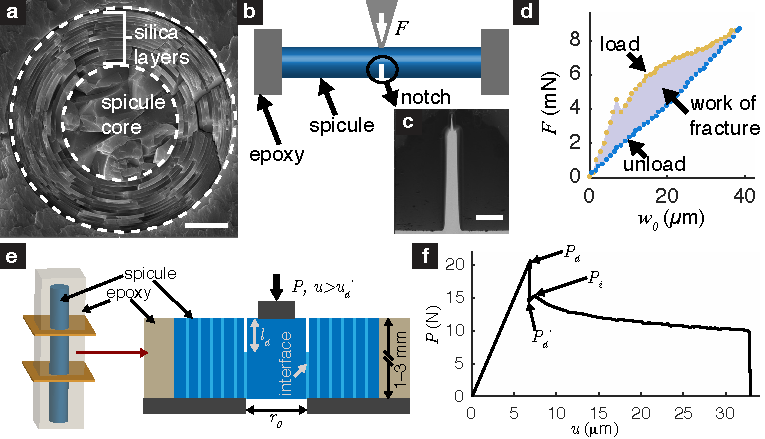
\includegraphics[width=\textwidth]{Figures/spicule/Layer_spicule_ver11.pdf}
            \caption{\footnotesize Measurement of the mechanical properties and behavior of spicules. (a) A SEM image of a \textit{E. aspergillum} spicule's cross-section showing its layered architecture. The scale bar measure 10 $\mu$m. (b) The three-point bending configuration used for the fracture tests described in A2.T2. The spicule is encastered at both ends with epoxy. A wedge-like indenter applies a force $F$ midway along the spicule's length perpendicular to its axis. (c) SEM micrograph of a notch cut in a spicule using FIB milling. The scale bar measures 500 nm. (d) The load-displacement response of a notched spicule (shown schematically in (b)). (e) Configuration of the the proposed cylinder push-out test. A spicule is embedded in epoxy, and cross-sectioned along the orange planes. The silica cylinders from the cross-section are mechanically supported from below and the core is pushed from above (shown in gray). The light blue lines indicate the interfaces between silica cylinders and between the first cylinder and the core. The initial interface crack with length $l_d$ is marked. (f) A typical load-displacement response obtained from a fiber push-out test (data obtained from~\cite{bright1989interfacial}).}
            \label{f:exp}
        \end{figure}
        %
        This configuration will freeze the relative motion of all weak interfaces except the first one between the core and its adjacent silica cylinder.
        %
        Thus, the core and the silica cylinders are analogous to the fiber and matrix, respectively, in the fiber push-out test~\cite{marshall1984indentation}.

        We will adapt the mechanical testing system, which we use to perform the bending tests (A2.T2), to perform the cylinder push-out test. During the test we will measure the applied force and indenter displacement.
        %
        We have made preliminary estimates of the force and displacement ranges needed for this test and found that our modified testing system will be able to perform the cylinder push-out test with 50 nm displacement resolution and 4 $\mu$N force resolution.

        A typical load-displacement curve from a fiber push-out test performed on a silicon carbide fiber reinforced composite is shown in Figure~\ref{f:exp} (f).
        %
        Initially, the applied force increases linearly with indenter displacement.
        %
        The abrupt drop in force from $P_d$ to $P_d^\prime$ corresponds to the formation of a crack along the fiber-matrix interface shown schematically in Figure~\ref{f:exp} (e).
        %
        Upon further loading, the  applied force again increases until it reaches $P_i$, at which point the crack begins to propagate along the length of the fiber.
        %
        If the length of the crack, $l_d$, at $P_d^\prime$ is large compared to the core radius, $r_0$, then the initiation force, $P_i$, is related to $g_{I}$ as $P_i=2\pi \sqrt{r_0^3 g_{cI} E^*}$~\cite{outwater1970fracture, kerans1991theoretical, liang1993mechanics}.
        %
        Knowing $E^*$ (from T.1.ii), and $r_0$ (from T.1.i), we will compute $g_{I}$ by measuring $P_i$ in the cylinder push-out test. However, after the test is completed we must verify that $l_d \gg r_0$.
        %
        We can compute $l_d$ by measuring the stiffness from the force-displacement response before and after crack nucleation, and choosing $l_d$ in a finite element model to match this stiffness ratio.
        %
        If $l_d$ is not much larger than $r_0$, then we will numerically compute the energy release rate for the cylinder push-out test using a finite element model in order to obtain $g_I$~\cite{moran1987crack}.

    \paragraph{A2.T2: Characterize the spicules' failure behavior}
      We will characterize the spicules' failure behavior by measuring the load-displacement response of a notched spicule in a three-point bending fracture test.
      %
      The PI has designed and built a mechanical testing system that is capable of performing the fracture tests with 200 nm displacement resolution and 20 $\mu$N force resolution \cite{monn2017enhanced,monn2017JoVE}. The system's design is based on that of an Atomic Force Microscope (AFM). The PI has considerable experience using the AFM for performing mechanical tests~\cite{kesariPML, kesariThesis} and has already performed three-point bending tests on spicules without notches using this custom-built system \cite{monn2017enhanced,monn2017JoVE,monn2017new}.
      %
      In the proposed tests, we will cut notches in the spicules in order to match the initial damaged state of the spicules in the experiments with the simulations. Through our preliminary research we were able to successfully create 5--25 $\mu$m long notches with a sharpness of approximately 100 nm using focused ion beam milling (see Figure~\ref{f:exp} (c)).

      Preliminary results from a bending fracture test performed on a notched spicule are shown in Figure~\ref{f:exp} (d). The applied force, $F$, and load-line displacement, $w_0$, are measured as the spicule is loaded in the configuration shown in Figure~\ref{f:exp} (b). The spicule is first loaded (yellow points) until a crack eminating from the notch root propagates completely across the spicule's cross-section. The spicule is then unloaded (blue points), and the area between the loading an unloading branches (shown in purple) constitutes the total energy dissipated by the fracture process.

    \paragraph{A2.T3: Compare the measurements to the aRVFT tool's predictions}
      We have designed the experiments and simulations so that the geometry, internal architecture, initial damage condition, and material properties match as closely as possible. Thus, we can characterize the aRVFT's predictive capability by whether it is able to reproduce the measured load-displacement curves. Based on statistics from our initial un-notched bending measurements, we plan on testing 60 spicules harvested from four different \textit{E. aspergillum} skeletons.

      \begin{table}[H]
        \center
        \caption{Project timeline}
        \label{t:timeline}
        \rowcolors{1}{lightgray}{white}
        \begin{tabular}{clll}
          \hline
          Task\textbackslash Year & 1 &  2 &  3 \\
          \hline
          A1 & T1 & T2 &  \\
          A2 & T1.i, T2 & T1.ii & T1.iii, T3 \\
          \hline
        \end{tabular}
      \end{table}

%%%%%%%%%%%%%%%%%%%%%%%%%%%%%%%%%%%%%%%%%%%%%%%%%%%%%%%%%%%%%%
%%%%%%%%%%%%%%%%%%%%%%%%%%%%%%%%%%%%%%%%%%%%%%%%%%%%%%%%%%%%%%
%%%%%%%%%%%%%%%%%%%%%%%%%%%%%%%%%%%%%%%%%%%%%%%%%%%%%%%%%%%%%%
\section{Broader impacts of the proposed work}
  \label{s:broaderimp}
  \paragraph{Collaboration with the Sci-Toons initiative}
    The Science Cartoons (Sci-Toons) initiative is a new strategy for communicating scientific research and concepts to a broad audience via storytelling, animation, high-quality multimedia and art. The initiative, part of broader impacts and education activities at Brown University's Science Center, engages STEM students, non-STEM students and faculty to create science animation videos that conceptualize and communicate science in an engaging and compelling manner to a broad range of audiences. The PI and his students will collaborate with the SciToons Creation Group (SCG), led by Dr. Oludurotimi Adetunji, Associate Dean for Undergraduate Research and Inclusive Science; and Executive Producer of the Brown University SciToons Initiative. The SCG consists of both STEM and non-STEM students, STEM domain content experts, voice over artists and animators.

    The Sci-Toons program's broader impacts goal of fostering greater understanding and appreciation of science in the general public is advanced by meshing communication and science, skills and interests of STEM and non-STEM majors. Four students, the PI and Dr. Adetunji are currently collaborating to produce a Sci-Toon animation that, through ``jargon-free'' language and storytelling, communicates the importance and impact of the results from the PI's recent publication~\cite{monn2015new} to a non-scientific audience. As part of the proposed project, the PI, in collaboration with SCG, will create one video per academic year for the next five years. The collaboration through this proposal will begin in Fall 2018. The videos will focus on the latest results from the research wing of the project. They will end by highlighting that the vast majority of the nature's designs are still unknown, and we will try to excite the viewers about the immense possibilities that the discovery of such designs would create for science and engineering. Funds to support the PI's future collaboration with the Sci-Toons initiative are requested as part of the budget (see Budget Justification). \emph{Evaluation}: The viewing impacts of Sci-Toons videos are gauged by monitoring the number and geographic distribution of views the videos generate using google analytics data. Prior Sci-Toons videos have been viewed in over 180 countries. Examples of completed Sci-Toons can be viewed on the Sci-Toons' YouTube channel.

    In addition to the Sci-Toons YouTube channel and a dedicated website, the Sci-Toons videos are distributed via a variety of social media platforms, such as Twitter (@Sci\_Toons) and Facebook. The Sci-Toons videos will also be posted on the PI's lab website. The website will be set up so that viewers can post comments and questions about the videos. The PI and his students will host a monthly virtual discussion group on Google Hangouts and address the posted comments and questions live. The PI will use the Sci-Toons videos in the undergraduate courses he teaches at Brown, such as Advanced Engineering Mechanics (ENGN 1370) and Advanced Engineering Optimization (ENGN 1950), which share the elements of solid and structural mechanics, and optimization principles with the topics that will be highlighted in the videos. The PI will also encourage his colleagues at Brown and other universities to use the videos in introductory engineering courses and in courses related to mechanics and optimization. \emph{Evaluation}: The videos' impact and utility in the classroom with be gauged by using the end of course student feedback form.

  \paragraph{Collaboration with SPIRA}
    SPIRA is a four week camp hosted at Brown every summer for high school age girls to explore engineering. For the past three years, the PI and his students have been collaborating with SPIRA in order to encourage young women to pursue education in STEM fields by exposing them to interesting applications of engineering. The camp is free to those who attend and often attracts students from underrepresented minorities.  Over the course of the proposed project, every summer, the PI and the students associated with the project will design and organize talks, workshops and competitions for the SPIRA participants. These activities will be tailored to make the participants aware of the wide range of exciting opportunities that are only recently becoming available to engineers, and through this awareness attract them to science and engineering. \emph{Talks:} Some of the past talks have been  ``Better materials through micro-scale mechanical design'' and and ``Bio-inspired engineering: why should we listen to nature.'' These talks were focused on the importance of bio-inspired materials to the future of mechanical engineering. Future talks will have a similar focus. The new results from the research component of the project will be used to enhance the quality of the talks. Following the talk, the students will be given a tour of PI's lab during which the presented research will be further explained using  physical examples and  practical demonstrations. \emph{Lab tour and workshop:} During the lab tour, the PI and his students will also explain the operating principles behind the different lab equipment. Last year's workshop was titled, "Hidden genius: a closer look at nature's architecture.'' In it, the participants examined spicules from the \textit{E. aspergillum} sponge as well as other biomaterials.  Pictures from  last  year's lab tour and workshop are shown in Figure~\ref{f:outreach}. The first workshop that will be held as part of the project is tentatively titled, ``Engineering Principles in Nature''.  In it, the PI's team and the participants will discuss the size, form, and function relationships in SBs, such as mammalian bones, eggshells, gecko's feet and the venus fly trap. \emph{Competition:} The competitions will give the participants an opportunity to learn through hands-on practice and experimentation. A competition under development for this project's SPIRA activities is tentatively titled ``Soft landing: better materials for tomorrow's helmets and cars''. In the competition the participants will be asked to construct a structure for cushioning the fall of a dropped egg by taking inspiration from nature. The student teams will be supplied with various materials and given access to the microscope in the PI's lab. Funds to organize this new competition in collaboration with SPIRA are requested as part of the budget (see Budget Justification). \emph{Evaluation:} The effectiveness of the planned SPIRA lectures, tutorials, and competitions will be gauged using exit interviews. The students' feedback will also be solicited by encouraging them to post comments and suggestions on the SPIRA section of the PI's website.

    \begin{figure}[h]
      \centering
      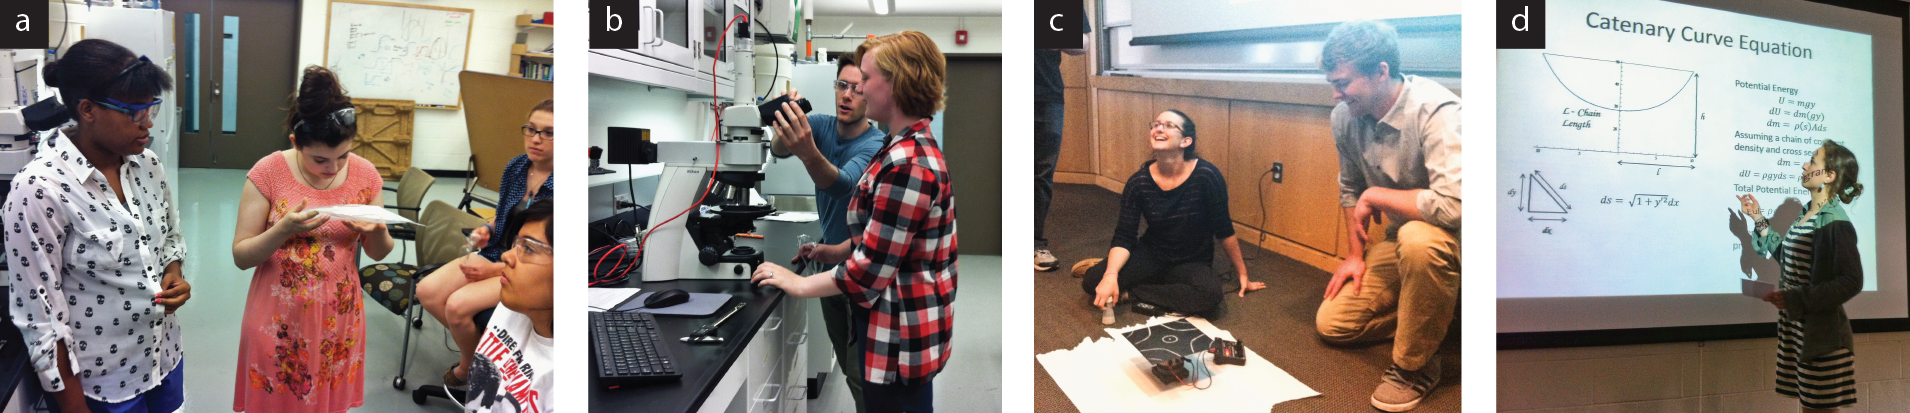
\includegraphics[width=\textwidth]{./Figures/SPIRA/OutreachFigure.png}
      \vspace{-10pt}
      \caption{\footnotesize (a)--(b) SPIRA students and (c)--(d) undergraduates from the PI's courses taking part in activities that were designed using the output from the PI's research program. The activities included several examples of how mechanics of materials research is enabling engineers to solve critical societal problems.}
      \label{f:outreach}
    \end{figure}

%%%%%%%%%%%%%%%%%%%%%%%%%%%%%%%%%%%%%%%%%%%%%%%%%%%%%%%%%%%%%%
%%%%%%%%%%%%%%%%%%%%%%%%%%%%%%%%%%%%%%%%%%%%%%%%%%%%%%%%%%%%%%
%%%%%%%%%%%%%%%%%%%%%%%%%%%%%%%%%%%%%%%%%%%%%%%%%%%%%%%%%%%%%%
\section{Results from prior NSF support}
  \label{s:priorfund}
  CMMI-1562656: ``Emergence of New Properties at the Large-Scale on Elastic Surfaces due to  Small-Scale Adhesion and Waviness,'' \$375,000, 03/01/2016 -- 02/28/2019. \textbf{Intellectual merit} The objective of this research is to understand how contact interactions between two surfaces at the micro-scale manifest as friction-like behavior at the macro-scale. Specifically, we relate friction at the macro-scale to dissipative mechanisms acting at the micro-scale that are activated by both adhesion and surface roughness. Through a synergistic combination of theoretical analysis, computer modeling, and experiments we will develop a rigorous mechanical theory governing the relationship between friction, adhesion, and surface roughness. A better understanding of this relationship could lead to advances in pick-and-place technology, MEMS, and biomimetic climbing robots. Four peer reviewed journal articles have been produced under this award so far, and three others are currently in preparation. Additionally, results from these articles have been disseminated through six conference presentations. As per the Data Management Plan for this award, computer code, experimental data, and theoretical results are made available through the Dropbox cloud storage system. \textbf{Broader impacts} Five graduate students (Wenqiang Fang, Weilin Deng, Michael Monn, Jarod Ferreira, Jianzhe Yang), and one undergraduate student (Christopher Owen-Elia) have worked on projects supported by this award. Two masters theses titled ``Adhesive contact experiments with non-linear model fitting''  and ``Deep indentation contact experiments with nonlinear model fitting'' have been completed by Jarod Ferreira and Jianzhe Yang, respectively, under the supervision of the PI. Finally, the PI has worked with the SciToons initiative at Brown University to create the first of a series of animated videos with a focus on bio-inspired engineering. The PI's collaboration with SciToons will be used to communicate research results to the STEM-interested public.

%%%%%%%%%%%%%%%%%%%%%%%%%%%%%%%%%%%%%%%%%%%%%%%%%%%%%%%%%%%%%%
%%%%%%%%%%%%%%%%%%%%%%%%%%%%%%%%%%%%%%%%%%%%%%%%%%%%%%%%%%%%%%
%%%%%%%%%%%%%%%%%%%%%%%%%%%%%%%%%%%%%%%%%%%%%%%%%%%%%%%%%%%%%%
\clearpage
\setcounter{page}{1}
\pagestyle{plain}
\bibliography{nsfCareer}

%%%%%%%%%%%%%%%%%%%%%%%%%%%%%%%%%%%%%%%%%%%%%%%%%%%%%%%%%%%%%%
%%%%%%%%%%%%%%%%%%%%%%%%%%%%%%%%%%%%%%%%%%%%%%%%%%%%%%%%%%%%%%
%%%%%%%%%%%%%%%%%%%%%%%%%%%%%%%%%%%%%%%%%%%%%%%%%%%%%%%%%%%%%%
\end{document}
